\documentclass[aps,pre,superscriptaddress,twocolumn,longbibliography,10pt]{revtex4-2}

\usepackage{graphicx}
\usepackage{amsmath}
\usepackage{dcolumn}
\usepackage{bm}
\usepackage{epstopdf}
\usepackage{algorithm}
\usepackage{algpseudocode}
\usepackage[colorlinks]{hyperref}
\usepackage{amsmath,amsthm,amssymb}
\usepackage{epsfig}
\usepackage{mathrsfs}
\usepackage{multirow}
\usepackage[all]{xy}
\usepackage{pbox}
\usepackage{verbatim}
\usepackage{braket}
\usepackage{mathtools}
\usepackage{tikz}
\usepackage{xcolor}
\usepackage{xfrac}
\usepackage{cleveref}
\usepackage[sort&compress]{natbib}

% Template below: replace 'initials' with your initials
% \newcommand{\initials}[1]{{\color{magenta}{\bf [INITIALS: KR]}}}
% Custom Commands
\newcommand{\singlefigure}{0.45\textwidth}


\begin{document}

\title{How to get escorted out of the casino, with Reinforcement Learning}

% AUTHORS
\author{Kieran Rudd}
\email{efykr2@nottingham.ac.uk}
\affiliation{School of Physics and Astronomy, University of Nottingham, Nottingham, NG7 2RD, UK}
\author{Michael Gamston}
\email{ppxmg5@nottingham.ac.uk}
\affiliation{School of Physics and Astronomy, University of Nottingham, Nottingham, NG7 2RD, UK}
\author{Scott Underdown}
\email{ppxsu1@nottingham.ac.uk}
\affiliation{School of Physics and Astronomy, University of Nottingham, Nottingham, NG7 2RD, UK}

\date{\today}

\begin{abstract}
    Note: use plain text. \\
Can prob just use AI to assist in this once done. 
\end{abstract}

\maketitle

\section{Introduction}

Blackjack, also known as twenty-one, is the most widely played casino game in the world, largely due to its simple game structure in which a player attempts to get the highest score by drawing cards from a deck. With its long history, various strategies for increasing a players chance of winning, such as card counting, are commonplace. Whilst an optimum strategy for blackjack has been known by statisticians for decades, by drawing on the expected value of future cards \cite{Baldwin01091956}, training an intelligent agent to learn the optimum strategy is an approach not as often taken. Using intelligent agents like this is known within machine learning communities as 'reinforcement learning'. The advantage of taking a reinforcement learning approach in this circumstance is rooted in the stochastic nature of blackjack, in which long term reward is prioritized. Additionally, its theorem proving nature offers extra insight, i.e., it can validate or indicate mathematical frameworks behind a system \cite{bidi2023reinforcementlearningcontroltheory}. 

\smallskip
Reinforcement Learning is a subfield of machine learning concerned with teaching an 'agent' to find an optimal set of moves - optimal policy - in the context of a wider system. The foundational components compose a policy - mapping possible states to possible actions, a reward signal - defining the agent's goal, an environment - which the agent interacts with, and a value function - indicating the long-term desirability of a sequence of states. Probabilistic reinforcement learning incorporates uncertainty into the decision-making process. Markov Decision Processes (MDP) inherently involve probabilities by modelling state transitions and reward distributions. A reinforcement learning task is considered a MDP if it satisfies the Markov property, defined as the exclusive reliance of the likelihood of changing to a specific state on the present state and elapsed time, and not on previous states \cite{10.5555/3312046}.

%Probabilistic reinforcement learning extends traditional reinforcement learning by incorporating uncertainty into decision-making processes through probabilistic transitions between states and rewards. This approach is particularly useful in environments where outcomes are uncertain or stochastic. In the context of Markov Decision Processes (MDPs), PRL naturally fits because MDPs inherently involve probabilities: they model state transitions and reward distributions, allowing for optimal policies that account for these uncertainties. (GENERATED)


%Given a finite MDP with state \(s\) and action \(a\), the probability of each following state and reward pair is given by
% \begin{multline}
%     p(a',r|s,a)=\\\text{Pr}\{S_{t+1}=s',R_{t+1}=r|S_t=s,A_t=a\}.
% \end{multline}
% Which entirely specifies the dynamics of the system.

\smallskip
There are many variations to Blackjack, typically involving multiple players and a dealer, but for the purposes of this project a stylized version with a single player and a passive dealer was played. The game uses a standard deck of cards with numerical values equal to their number for cards 2-10, and equal to 10 for Jacks, Queens, and Kings. Aces are valued at 11 unless the sum of the cards in hand exceeds 21, in which case they are valued at 1. The sequence of play is as follows:
\begin{enumerate}
    \item A card is dealt to the player with value \(C_1\).
    \item For \(n\) iterations, or until a total score of 21 is exceeded, the player can make one of two choices;
    \begin{enumerate} 
        \item Stick, and end the game.
        \item Hit, and receive another card with value \(C_{n+1}\).
    \end{enumerate}
    \item The final score is calculated using
        \begin{equation} \label{eq: Score}
            S= 
            \begin{cases}
                (\sum C_n)^2 & \text{if } \sum C_n \le 21\\
                0            & \text{if } \sum C_n >   21\\
            \end{cases}
        \end{equation}
\end{enumerate}
\smallskip
To approach this problem, two situations were considered. Infinite, in which the pile of cards being drawn from is infinite, meaning the probability of each card being drawn is equal, and finite, in which the pile of cards being drawn from is finite, meaning unequal probabilities. These two approaches were taken to provide a broad spectrum of results. This paper details the methodology taken for both problem situations, the results of each in context of an optimal result, and a conclusion on the efficacy of this approach.
\section{Methodology}

In training an agent to play Blackjack, an iterative Q-Learning approach has been taken. Watkins' Q-Learning aims to learn the optimal 'q-value' for given state-action pairs in an environment, i.e., the respective value of making a certain move in a certain environmental state. ... further description

This approach was selected because it does not require direct 

The Bellman's equations for Q-Learning is defined as,
\begin{multline}
    Q_{new}(s,a)=Q_{old}(s,a)+\\\alpha(\underbrace{R(s,a)+\gamma MaxQ(s',a')-Q_{old}(s,a)}_{\mathclap{\text{Temporal Difference}}})
\end{multline}
Where \( s, a \) are the current state and action,  \( s', a' \) are the next state and action, \( \alpha \) is the learning rate, \( \gamma \) is the discount factor, \( R(s,a) \) is the reward received after taking action \( a \) in state \( s \), and \( Q(s,a) \) is the q-value for the state-action pair. 



Temporal difference somewhere. 

Explain Q-tables and the inner functionality of learning in conjunction with the temporal difference. 

alpha and how it decreases


To train the model, Python and its basic libraries were employed, i.e., no machine learning libraries like Keras or Tensorflow. 

\subsection{Infinite}

In the "infinite" situation, the probability of each card being drawn is equal, so retaining prior knowledge of cards drawn poses no advantage, i.e., this situation is purely probabilistic. 

The Q-table for the infinite situation is composed of the dimensions, 
\begin{itemize}
    \item Card count: 2-20
    \item Held ace: Y/N
    \item Action: Hit/Stick
\end{itemize}


\subsection{Finite}

In the 'finite' situation, cards were drawn from a pile of finite number, meaning that the probability of drawing respective cards changed as the game progressed. This posed a new challenge which could ideally be solved by providing the agent with all previously dealt cards, from which it could learn to predict the probabilities of newly dealt cards, and so, how risk-adverse it should play. However, doing so would be at great computational cost, where the Q-table would need to incorporate the dimensions previously described, in addition to some combination of previously dealt cards. 

To strike a balance between accuracy and potential advantage, the probability of 

... consider other methods (like card counting)

? average of recived cards???
\section{Results}

Here, one can display figures, such as in \Cref{fig:example}.

\begin{figure}
    \centering
    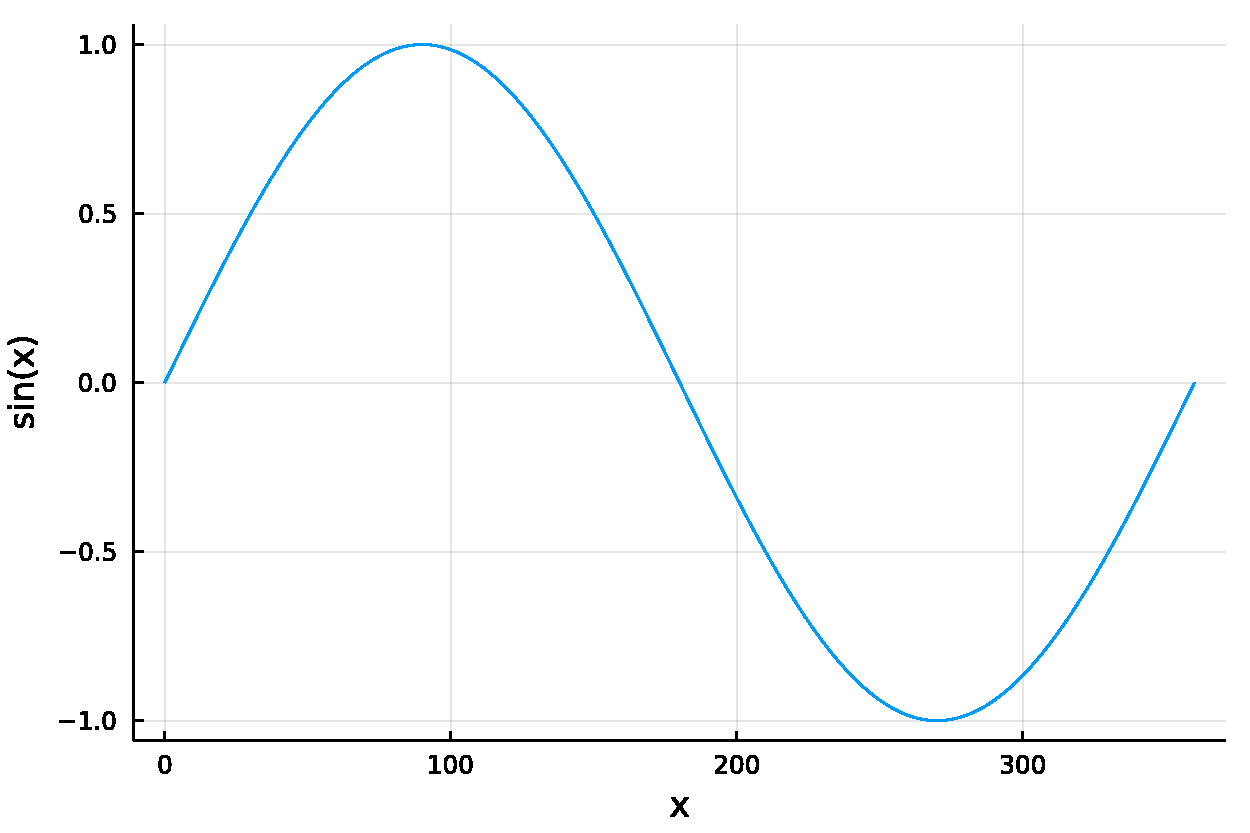
\includegraphics[width=\singlefigure]{figures/example.pdf}
    \caption{\label{fig:example} Shows an example of a figure.}
\end{figure}

Ideas;
* policy
* ideal policy (needs mathematical modelling)
* learning rates (and alpha rates?) : absolute and relative changes - derivatives
* differences between held ace and no held ace
* actual score (moving average?)
\section{Conclusions}
\dots
4 pages, not including references. Allow space for abstract.

This paper successfully presents a Q-learning, reinforcement learning approach to blackjack's optimal policy - the set of best rewarding moves in game state. blah blah

\bibliographystyle{apsrev4-2}
\bibliography{references}
\appendix

\end{document}